\subsection{Longitudinal variability}

Observations of Titan taken from a near polar point of view offer a unique way to study the evolution of
the detached haze with a large coverage in longitude and within in a small range of latitudes. It allows
first to check the homogeneity of the haze in longitude, and it also allows us to extend our previous
observations between the dawn/dusk sides with a local time coverage between 6:00 and 18:00.

\begin{figure}[!ht]
    \centering
    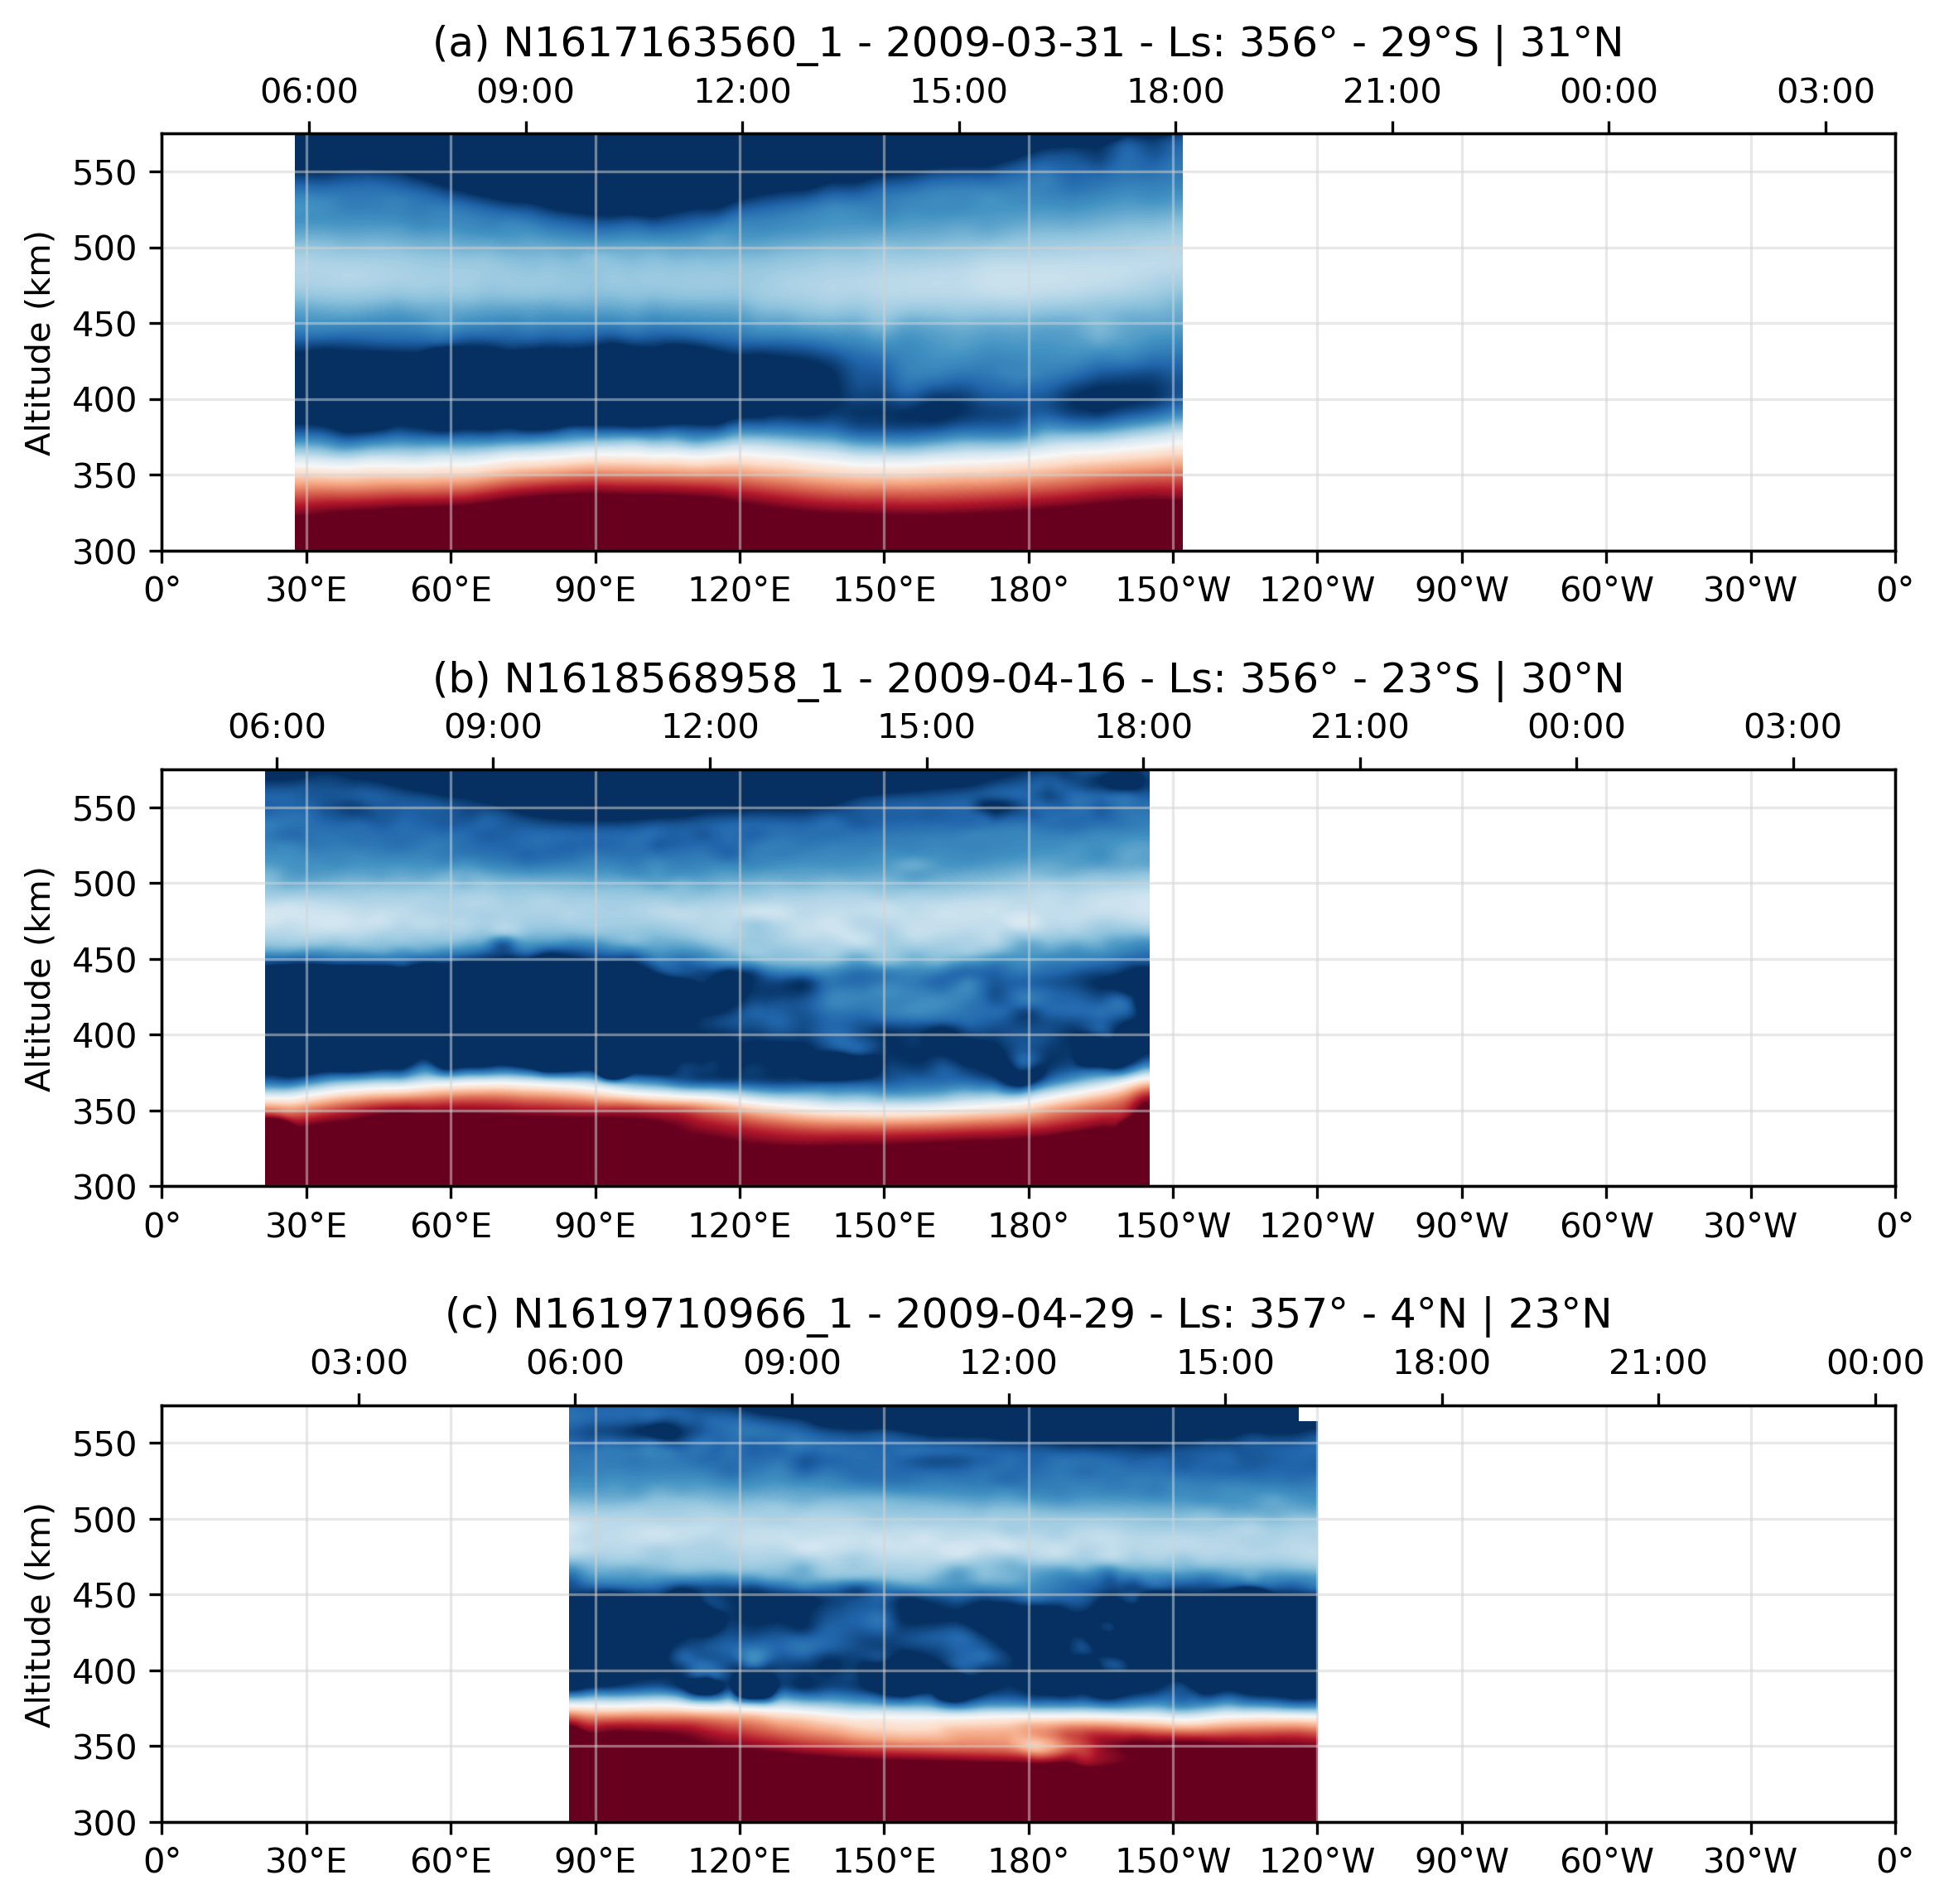
\includegraphics[width=.8\textwidth]{Fig/Lon_variability.png}
    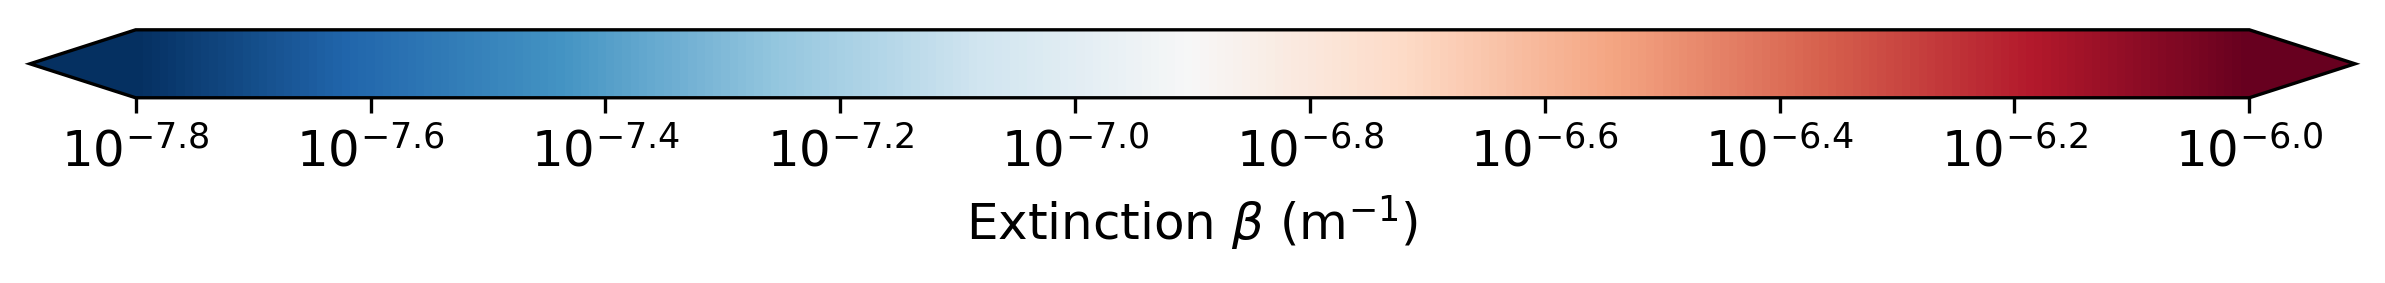
\includegraphics[width=.5\textwidth]{Fig/Extinction_colorbar.png}\vspace{-.3cm}
    \caption{The panels show the map of the haze extinction as a function of the longitude and the local
    for a set of 3 images taken in March and April 2009 ($L_s=\ang{356}$). The latitude range covered is
    also indicated for each image.}
    \label{fig:lon_variability}
\end{figure}

We analyze a set of three images taken sequentially within a month interval. The first observation
was performed the 29$^{th}$ of March 2009 (Fig.~\ref{fig:lon_variability}a) during the collapse of the detached
haze layer. Two other observations were made only two weeks and one month later, with the same geometry
(Figs.~\ref{fig:lon_variability}b, \ref{fig:lon_variability}c). The detached haze layer is
located at 470 km at all the longitudes. Inside the depletion region, we notice a plume of haze
between 400 and 440 km and between \ang{140}E and \ang{210}E. In mid-April, the plume is located between
\ang{120}E and \ang{200}E and between 375 and 425 km. It appears disconnected and settling from the detached
layer, which remains at 470 km. At the end of April, we now see the extension around 410 km and it
is spread from \ang{110}E and \ang{180}E. This separated aerosols plume is almost connected with the main haze.

This feature is not correlated with the local time but remains about at the same longitude and drifts slowly
toward the West. This would correspond to a retrograde motion of about 0.6 m/s. Another solution would be
prograde motion of 6.6 m/s, in phase with the sampling of 15 terrestrial days. The vertical speed, assuming
that the aerosol cloud drop from 400 km to 375 km in one month would be $10^{-3}$ m/s. We also can remark a
modulation in the extinction and in the geometrical thickness of both the detached haze layer and the main
haze. In the last image, only the geometrical thickness is modulated and not the haze extinction.

These observations show that the haze layer is not completely homogeneous in longitude and have some
fluctuations in extinction and in geometry.
% NOTE: [PR] I think that the curve  $\beta$ .vs. Longitude and Thickness .vs. Longitude would be useful here to have a quantitative view on these variations. At least, we should give an numerical value for the order of magnitude of these variations in the DHL.
It also strengthen the idea that space and time variations, as in observations previously discussed,
can not be distinguished without additional observations. The dawn/dusk differences and the short term variations,
presented in the two previous subsections, could be due to longitudinal effect rather than to time variations.
Therefore, with the results of this section, we stress that the longitude inhomogeneities should be kept
in mind when discussing and comparing latitudinal maps of detached haze layer.